\documentclass[11pt]{article}\usepackage[]{graphicx}\usepackage[]{color}
%% maxwidth is the original width if it is less than linewidth
%% otherwise use linewidth (to make sure the graphics do not exceed the margin)
\makeatletter
\def\maxwidth{ %
  \ifdim\Gin@nat@width>\linewidth
    \linewidth
  \else
    \Gin@nat@width
  \fi
}
\makeatother

\definecolor{fgcolor}{rgb}{0.345, 0.345, 0.345}
\newcommand{\hlnum}[1]{\textcolor[rgb]{0.686,0.059,0.569}{#1}}%
\newcommand{\hlstr}[1]{\textcolor[rgb]{0.192,0.494,0.8}{#1}}%
\newcommand{\hlcom}[1]{\textcolor[rgb]{0.678,0.584,0.686}{\textit{#1}}}%
\newcommand{\hlopt}[1]{\textcolor[rgb]{0,0,0}{#1}}%
\newcommand{\hlstd}[1]{\textcolor[rgb]{0.345,0.345,0.345}{#1}}%
\newcommand{\hlkwa}[1]{\textcolor[rgb]{0.161,0.373,0.58}{\textbf{#1}}}%
\newcommand{\hlkwb}[1]{\textcolor[rgb]{0.69,0.353,0.396}{#1}}%
\newcommand{\hlkwc}[1]{\textcolor[rgb]{0.333,0.667,0.333}{#1}}%
\newcommand{\hlkwd}[1]{\textcolor[rgb]{0.737,0.353,0.396}{\textbf{#1}}}%
\let\hlipl\hlkwb

\usepackage{framed}
\makeatletter
\newenvironment{kframe}{%
 \def\at@end@of@kframe{}%
 \ifinner\ifhmode%
  \def\at@end@of@kframe{\end{minipage}}%
  \begin{minipage}{\columnwidth}%
 \fi\fi%
 \def\FrameCommand##1{\hskip\@totalleftmargin \hskip-\fboxsep
 \colorbox{shadecolor}{##1}\hskip-\fboxsep
     % There is no \\@totalrightmargin, so:
     \hskip-\linewidth \hskip-\@totalleftmargin \hskip\columnwidth}%
 \MakeFramed {\advance\hsize-\width
   \@totalleftmargin\z@ \linewidth\hsize
   \@setminipage}}%
 {\par\unskip\endMakeFramed%
 \at@end@of@kframe}
\makeatother

\definecolor{shadecolor}{rgb}{.97, .97, .97}
\definecolor{messagecolor}{rgb}{0, 0, 0}
\definecolor{warningcolor}{rgb}{1, 0, 1}
\definecolor{errorcolor}{rgb}{1, 0, 0}
\newenvironment{knitrout}{}{} % an empty environment to be redefined in TeX

\usepackage{alltt}
\usepackage{amsmath}
\usepackage{amssymb}
\usepackage{geometry}
\usepackage{graphicx}
\usepackage{bm}
\usepackage{url}
\usepackage{enumerate}
\usepackage{hyperref}
\IfFileExists{upquote.sty}{\usepackage{upquote}}{}
\begin{document}

\setlength\parindent{0pt}

\large \textbf{Lab 3: Polynomial Regression}\\
\normalsize STAT 632, Spring 2020\\

Note: This lab borrows from Ch. 3, pp. 115-117 of \emph{An Introduction to Statistical Learning}.\\

A polynomial regression model can be written as 
$$ Y = \beta_0 + \beta_1 x + \beta_2 x^2 + \cdots + \beta_p x^p + e$$

One way to choose $p$ is to keep adding terms until the added (highest order) term is no longer significant.  It is recommended to keep all lower order terms in the model, even if they are not statistically significant.  For example, if we fit a cubic model, then we should keep that $x$ and $x^2$ terms in the model.\\  

As an example, we consider a data set called \texttt{Boston} on housing values and other information about Boston suburbs.  The data set is from the \texttt{MASS} package.  We are interested in fitting a polynomial regression model with $Y=$ \texttt{medv} as the response and $x=$ \texttt{lstat} as the predictor.  The variable \texttt{medv} is the median house value (in \$1000), and \texttt{lstat} is the percent of households with low socioeconomic status.  A scatterplot of the data is shown below.

\begin{knitrout}
\definecolor{shadecolor}{rgb}{0.969, 0.969, 0.969}\color{fgcolor}\begin{kframe}
\begin{alltt}
\hlkwd{library}\hlstd{(MASS)}
\hlkwd{library}\hlstd{(ggplot2)}
\hlkwd{ggplot}\hlstd{(}\hlkwc{data}\hlstd{=Boston,} \hlkwd{aes}\hlstd{(lstat, medv))} \hlopt{+} \hlkwd{geom_point}\hlstd{(}\hlkwc{size}\hlstd{=}\hlnum{0.5}\hlstd{)}
\end{alltt}
\end{kframe}
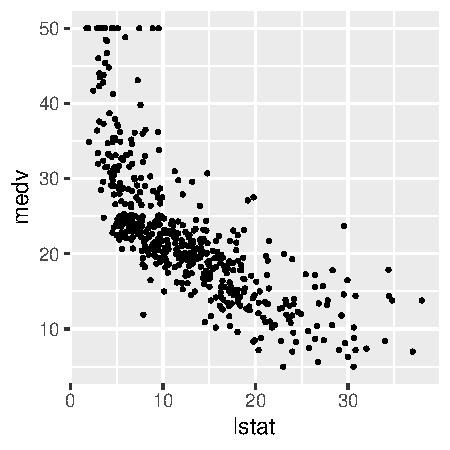
\includegraphics[width=\maxwidth]{figure/unnamed-chunk-1-1} 

\end{knitrout}
\clearpage

Let's start with a quadratic polynomial model:
\begin{knitrout}
\definecolor{shadecolor}{rgb}{0.969, 0.969, 0.969}\color{fgcolor}\begin{kframe}
\begin{alltt}
\hlstd{lm2} \hlkwb{<-} \hlkwd{lm}\hlstd{(medv} \hlopt{~} \hlstd{lstat} \hlopt{+} \hlkwd{I}\hlstd{(lstat}\hlopt{^}\hlnum{2}\hlstd{),} \hlkwc{data} \hlstd{= Boston)}
\hlkwd{summary}\hlstd{(lm2)}
\end{alltt}
\begin{verbatim}
## 
## Call:
## lm(formula = medv ~ lstat + I(lstat^2), data = Boston)
## 
## Residuals:
##      Min       1Q   Median       3Q      Max 
## -15.2834  -3.8313  -0.5295   2.3095  25.4148 
## 
## Coefficients:
##              Estimate Std. Error t value Pr(>|t|)    
## (Intercept) 42.862007   0.872084   49.15   <2e-16 ***
## lstat       -2.332821   0.123803  -18.84   <2e-16 ***
## I(lstat^2)   0.043547   0.003745   11.63   <2e-16 ***
## ---
## Signif. codes:  0 '***' 0.001 '**' 0.01 '*' 0.05 '.' 0.1 ' ' 1
## 
## Residual standard error: 5.524 on 503 degrees of freedom
## Multiple R-squared:  0.6407,	Adjusted R-squared:  0.6393 
## F-statistic: 448.5 on 2 and 503 DF,  p-value: < 2.2e-16
\end{verbatim}
\end{kframe}
\end{knitrout}
The near-zero p-value indicates that quadratic term is significant and should be included in the model.\\

To fit a cubic regression model, we can add a predictor of the form \texttt{I(X\^{}3)}.  However this can start to get cumbersome as we continue to add higher order terms.  A better approach is to use the \texttt{poly()} function. By default \texttt{poly()} uses what are called orthogonal polynomials (this means the columns of the design matrix are orthogonal).  This can improve numeric stability.  However, if we set the argument \texttt{raw=TRUE}, then \texttt{poly()} will do the same thing as if we had manually entered the terms using \texttt{I()}.  Either way, the predictions will be the same when using \texttt{predict()} (it's just the coefficients that change when using orthogonal polynomials).\\
\clearpage

Moving forward we consider higher order terms:
\begin{knitrout}
\definecolor{shadecolor}{rgb}{0.969, 0.969, 0.969}\color{fgcolor}\begin{kframe}
\begin{alltt}
\hlstd{lm3} \hlkwb{<-} \hlkwd{lm}\hlstd{(medv} \hlopt{~} \hlkwd{poly}\hlstd{(lstat,} \hlnum{3}\hlstd{),} \hlkwc{data}\hlstd{=Boston)}
\hlstd{lm4} \hlkwb{<-} \hlkwd{lm}\hlstd{(medv} \hlopt{~} \hlkwd{poly}\hlstd{(lstat,} \hlnum{4}\hlstd{),} \hlkwc{data}\hlstd{=Boston)}
\hlstd{lm5} \hlkwb{<-} \hlkwd{lm}\hlstd{(medv} \hlopt{~} \hlkwd{poly}\hlstd{(lstat,} \hlnum{5}\hlstd{),} \hlkwc{data}\hlstd{=Boston)}
\hlstd{lm6} \hlkwb{<-} \hlkwd{lm}\hlstd{(medv} \hlopt{~} \hlkwd{poly}\hlstd{(lstat,} \hlnum{6}\hlstd{),} \hlkwc{data}\hlstd{=Boston)}
\end{alltt}
\end{kframe}
\end{knitrout}

The p-values are significant up to the fifth order term.
\begin{knitrout}
\definecolor{shadecolor}{rgb}{0.969, 0.969, 0.969}\color{fgcolor}\begin{kframe}
\begin{alltt}
\hlkwd{summary}\hlstd{(lm5)}
\end{alltt}
\begin{verbatim}
## 
## Call:
## lm(formula = medv ~ poly(lstat, 5), data = Boston)
## 
## Residuals:
##      Min       1Q   Median       3Q      Max 
## -13.5433  -3.1039  -0.7052   2.0844  27.1153 
## 
## Coefficients:
##                  Estimate Std. Error t value Pr(>|t|)    
## (Intercept)       22.5328     0.2318  97.197  < 2e-16 ***
## poly(lstat, 5)1 -152.4595     5.2148 -29.236  < 2e-16 ***
## poly(lstat, 5)2   64.2272     5.2148  12.316  < 2e-16 ***
## poly(lstat, 5)3  -27.0511     5.2148  -5.187 3.10e-07 ***
## poly(lstat, 5)4   25.4517     5.2148   4.881 1.42e-06 ***
## poly(lstat, 5)5  -19.2524     5.2148  -3.692 0.000247 ***
## ---
## Signif. codes:  0 '***' 0.001 '**' 0.01 '*' 0.05 '.' 0.1 ' ' 1
## 
## Residual standard error: 5.215 on 500 degrees of freedom
## Multiple R-squared:  0.6817,	Adjusted R-squared:  0.6785 
## F-statistic: 214.2 on 5 and 500 DF,  p-value: < 2.2e-16
\end{verbatim}
\end{kframe}
\end{knitrout}
\clearpage

The p-value for the sixth order term is not significant, so there is no improvement by considering terms beyond \texttt{lstat}$^5$.
\begin{knitrout}
\definecolor{shadecolor}{rgb}{0.969, 0.969, 0.969}\color{fgcolor}\begin{kframe}
\begin{alltt}
\hlkwd{summary}\hlstd{(lm6)}
\end{alltt}
\begin{verbatim}
## 
## Call:
## lm(formula = medv ~ poly(lstat, 6), data = Boston)
## 
## Residuals:
##      Min       1Q   Median       3Q      Max 
## -14.7317  -3.1571  -0.6941   2.0756  26.8994 
## 
## Coefficients:
##                  Estimate Std. Error t value Pr(>|t|)    
## (Intercept)       22.5328     0.2317  97.252  < 2e-16 ***
## poly(lstat, 6)1 -152.4595     5.2119 -29.252  < 2e-16 ***
## poly(lstat, 6)2   64.2272     5.2119  12.323  < 2e-16 ***
## poly(lstat, 6)3  -27.0511     5.2119  -5.190 3.06e-07 ***
## poly(lstat, 6)4   25.4517     5.2119   4.883 1.41e-06 ***
## poly(lstat, 6)5  -19.2524     5.2119  -3.694 0.000245 ***
## poly(lstat, 6)6    6.5088     5.2119   1.249 0.212313    
## ---
## Signif. codes:  0 '***' 0.001 '**' 0.01 '*' 0.05 '.' 0.1 ' ' 1
## 
## Residual standard error: 5.212 on 499 degrees of freedom
## Multiple R-squared:  0.6827,	Adjusted R-squared:  0.6789 
## F-statistic: 178.9 on 6 and 499 DF,  p-value: < 2.2e-16
\end{verbatim}
\end{kframe}
\end{knitrout}

Next we plot the estimated fifth degree polynomial regression curve on the scatterplot.  We also add a confidence interval band (\texttt{ggplot2} does this by default).  
\begin{knitrout}
\definecolor{shadecolor}{rgb}{0.969, 0.969, 0.969}\color{fgcolor}\begin{kframe}
\begin{alltt}
\hlkwd{ggplot}\hlstd{(}\hlkwc{data}\hlstd{=Boston,} \hlkwd{aes}\hlstd{(lstat, medv))} \hlopt{+}
  \hlkwd{geom_point}\hlstd{(}\hlkwc{size}\hlstd{=}\hlnum{0.5}\hlstd{)} \hlopt{+}
  \hlkwd{stat_smooth}\hlstd{(}\hlkwc{method} \hlstd{=} \hlstr{'lm'}\hlstd{,} \hlkwc{formula} \hlstd{= y} \hlopt{~} \hlkwd{poly}\hlstd{(x,} \hlnum{5}\hlstd{))}
\end{alltt}
\end{kframe}
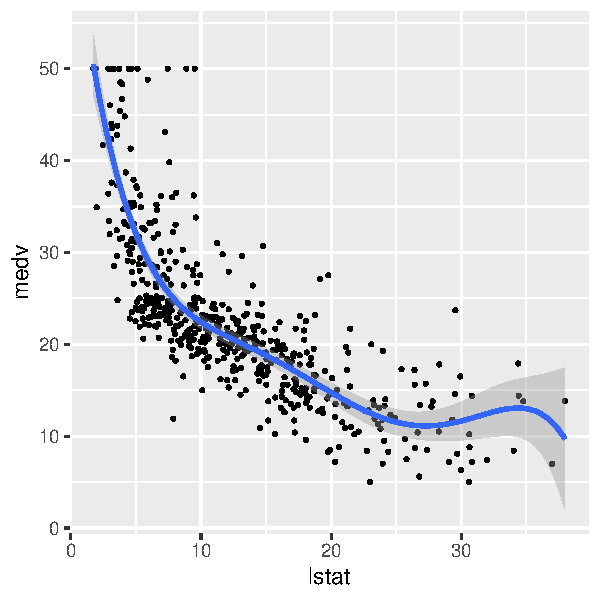
\includegraphics[width=\maxwidth]{figure/unnamed-chunk-6-1} 

\end{knitrout}

\vspace{20pt}
\Large
\textbf{Cross-validation}\\
\normalsize

The p-value approach suggested that we select the 5th degree polynomial regression model.  An alternative way of selecting the degree is to use cross-validation.  The idea is to split the data into two parts: a training set and a validation (or test) set.  We then estimate the models on the training set, and make predictions on the withheld validation set.  The models are then compared in terms of their root mean square prediction error:
$$ \text{RMSE} = \sqrt{\frac{1}{n_v} \sum_{i=1}^{n_v} (y_i - \hat{y_i})^2} $$
where $n_v$ is the number of observations in the validation set; and $y_i$ and $\hat{y}_i$ are the actual and predicted values for the $i^{th}$ observation in the validation set.  This approach will give us an idea of how well our models perform on out-of-sample data.
\clearpage

First, I wrote a function in R to compute the RMSE.  
\begin{knitrout}
\definecolor{shadecolor}{rgb}{0.969, 0.969, 0.969}\color{fgcolor}\begin{kframe}
\begin{alltt}
\hlstd{compute_rmse} \hlkwb{<-} \hlkwa{function}\hlstd{(}\hlkwc{y}\hlstd{,} \hlkwc{y_pred}\hlstd{) \{}
  \hlstd{n} \hlkwb{<-} \hlkwd{length}\hlstd{(y)}
  \hlkwd{sqrt}\hlstd{((}\hlnum{1} \hlopt{/} \hlstd{n)} \hlopt{*} \hlkwd{sum}\hlstd{((y} \hlopt{-} \hlstd{y_pred)}\hlopt{^}\hlnum{2}\hlstd{))}
\hlstd{\}}
\end{alltt}
\end{kframe}
\end{knitrout}

The Boston data set has $n=506$ observations (rows).  We randomly split the 506 observations into two sets, a training set containing 354 observations (70\% of the data), and a validation set containing 152 observations (30\% of the data).

\begin{knitrout}
\definecolor{shadecolor}{rgb}{0.969, 0.969, 0.969}\color{fgcolor}\begin{kframe}
\begin{alltt}
\hlkwd{set.seed}\hlstd{(}\hlnum{100}\hlstd{)}
\hlstd{n} \hlkwb{<-} \hlkwd{nrow}\hlstd{(Boston)}
\hlstd{train} \hlkwb{<-} \hlkwd{sample}\hlstd{(}\hlnum{1}\hlopt{:}\hlstd{n,} \hlkwc{size}\hlstd{=}\hlnum{354}\hlstd{)}

\hlstd{lm1_train} \hlkwb{<-} \hlkwd{lm}\hlstd{(medv} \hlopt{~} \hlstd{lstat,} \hlkwc{data}\hlstd{=Boston,} \hlkwc{subset}\hlstd{=train)}
\hlstd{lm2_train} \hlkwb{<-} \hlkwd{lm}\hlstd{(medv} \hlopt{~} \hlkwd{poly}\hlstd{(lstat,} \hlnum{2}\hlstd{),} \hlkwc{data}\hlstd{=Boston,} \hlkwc{subset}\hlstd{=train)}
\hlstd{lm3_train} \hlkwb{<-} \hlkwd{lm}\hlstd{(medv} \hlopt{~} \hlkwd{poly}\hlstd{(lstat,} \hlnum{3}\hlstd{),} \hlkwc{data}\hlstd{=Boston,} \hlkwc{subset}\hlstd{=train)}
\hlstd{lm4_train} \hlkwb{<-} \hlkwd{lm}\hlstd{(medv} \hlopt{~} \hlkwd{poly}\hlstd{(lstat,} \hlnum{4}\hlstd{),} \hlkwc{data}\hlstd{=Boston,} \hlkwc{subset}\hlstd{=train)}
\hlstd{lm5_train} \hlkwb{<-} \hlkwd{lm}\hlstd{(medv} \hlopt{~} \hlkwd{poly}\hlstd{(lstat,} \hlnum{5}\hlstd{),} \hlkwc{data}\hlstd{=Boston,} \hlkwc{subset}\hlstd{=train)}
\hlstd{lm6_train} \hlkwb{<-} \hlkwd{lm}\hlstd{(medv} \hlopt{~} \hlkwd{poly}\hlstd{(lstat,} \hlnum{6}\hlstd{),} \hlkwc{data}\hlstd{=Boston,} \hlkwc{subset}\hlstd{=train)}

\hlstd{rmse} \hlkwb{<-} \hlkwd{rep}\hlstd{(}\hlnum{0}\hlstd{,} \hlnum{6}\hlstd{)}
\hlstd{y_test} \hlkwb{<-} \hlstd{Boston}\hlopt{$}\hlstd{medv[}\hlopt{-}\hlstd{train]}
\hlstd{new_x} \hlkwb{<-} \hlkwd{data.frame}\hlstd{(}\hlkwc{lstat} \hlstd{= Boston}\hlopt{$}\hlstd{lstat[}\hlopt{-}\hlstd{train])}
\hlstd{y1_pred} \hlkwb{<-} \hlkwd{predict}\hlstd{(lm1_train,} \hlkwc{newdata} \hlstd{= new_x)}
\hlstd{rmse[}\hlnum{1}\hlstd{]} \hlkwb{<-} \hlkwd{compute_rmse}\hlstd{(y_test, y1_pred)}
\hlstd{y2_pred} \hlkwb{<-} \hlkwd{predict}\hlstd{(lm2_train,} \hlkwc{newdata} \hlstd{= new_x)}
\hlstd{rmse[}\hlnum{2}\hlstd{]} \hlkwb{<-} \hlkwd{compute_rmse}\hlstd{(y_test, y2_pred)}
\hlstd{y3_pred} \hlkwb{<-} \hlkwd{predict}\hlstd{(lm3_train,} \hlkwc{newdata} \hlstd{= new_x)}
\hlstd{rmse[}\hlnum{3}\hlstd{]} \hlkwb{<-} \hlkwd{compute_rmse}\hlstd{(y_test, y3_pred)}
\hlstd{y4_pred} \hlkwb{<-} \hlkwd{predict}\hlstd{(lm4_train,} \hlkwc{newdata} \hlstd{= new_x)}
\hlstd{rmse[}\hlnum{4}\hlstd{]} \hlkwb{<-} \hlkwd{compute_rmse}\hlstd{(y_test, y4_pred)}
\hlstd{y5_pred} \hlkwb{<-} \hlkwd{predict}\hlstd{(lm5_train,} \hlkwc{newdata} \hlstd{= new_x)}
\hlstd{rmse[}\hlnum{5}\hlstd{]} \hlkwb{<-} \hlkwd{compute_rmse}\hlstd{(y_test, y5_pred)}
\hlstd{y6_pred} \hlkwb{<-} \hlkwd{predict}\hlstd{(lm6_train,} \hlkwc{newdata} \hlstd{= new_x)}
\hlstd{rmse[}\hlnum{6}\hlstd{]} \hlkwb{<-} \hlkwd{compute_rmse}\hlstd{(y_test, y6_pred)}
\end{alltt}
\end{kframe}
\end{knitrout}

\begin{knitrout}
\definecolor{shadecolor}{rgb}{0.969, 0.969, 0.969}\color{fgcolor}\begin{kframe}
\begin{alltt}
\hlcom{# print RMSE vector}
\hlstd{rmse}
\end{alltt}
\begin{verbatim}
## [1] 6.134497 5.448901 5.274728 5.335416 5.014329 5.593054
\end{verbatim}
\begin{alltt}
\hlkwd{par}\hlstd{(}\hlkwc{mar}\hlstd{=}\hlkwd{c}\hlstd{(}\hlnum{4.5}\hlstd{,}\hlnum{4}\hlstd{,}\hlnum{1}\hlstd{,}\hlnum{1}\hlstd{))} \hlcom{# adjust margins}
\hlkwd{plot}\hlstd{(}\hlkwd{c}\hlstd{(}\hlnum{1}\hlopt{:}\hlnum{6}\hlstd{), rmse,} \hlkwc{xlab}\hlstd{=}\hlstr{"Degree of polynomial"}\hlstd{,} \hlkwc{ylab}\hlstd{=}\hlstr{"RMSE"}\hlstd{,} \hlkwc{type}\hlstd{=}\hlstr{'b'}\hlstd{)}
\end{alltt}
\end{kframe}
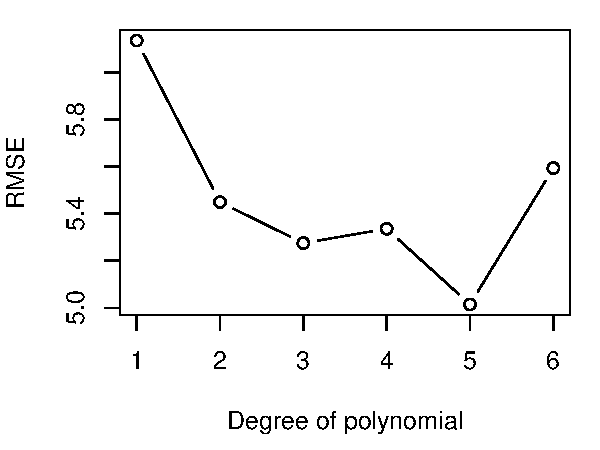
\includegraphics[width=\maxwidth]{figure/unnamed-chunk-9-1} 

\end{knitrout}

The cross-validation results agree with p-value approach, since the degree 5 polynomial has the lowest RMSE.\\ 

Note that it would have been better to write the code above as a \texttt{for-loop}.  Also, note that the validation set approach can be highly variable.  Another random split might select a different model.  There are more stable approaches like leave-one-out cross-validation and 10-fold cross-validation.  You can also take the average RMSE over several 70/30 splits of the data.
\clearpage

\large \textbf{Regression Splines}\\

\normalsize
We don't have to limit ourselves to just using polynomials to model nonlinearities.  In fact, one shortcoming of polynomial regression is that each point affects the fit globally; polynomials can also start to overfit the data when the degree $p$ is greater than 4. Regression splines are an alternative technique that fits polynomials locally.  That is, polynomial models (usually cubic) are fit piecewise to the data, under some constraints for continuity and smoothness.  \texttt{ggplot2} provides a convenient way to visualize and experiment with splines.  You can read more about regression splines in Chapter 7 of \emph{An Introduction to Statistical Learning}.  

\begin{knitrout}
\definecolor{shadecolor}{rgb}{0.969, 0.969, 0.969}\color{fgcolor}\begin{kframe}
\begin{alltt}
\hlkwd{ggplot}\hlstd{(}\hlkwc{data}\hlstd{=Boston,} \hlkwd{aes}\hlstd{(lstat, medv))} \hlopt{+}
  \hlkwd{geom_point}\hlstd{(}\hlkwc{size}\hlstd{=}\hlnum{0.5}\hlstd{)} \hlopt{+}
  \hlkwd{stat_smooth}\hlstd{(}\hlkwc{method} \hlstd{=} \hlstr{'lm'}\hlstd{,} \hlkwc{formula} \hlstd{= y} \hlopt{~} \hlstd{splines}\hlopt{::}\hlkwd{bs}\hlstd{(x,}\hlnum{7}\hlstd{))}
\end{alltt}
\end{kframe}
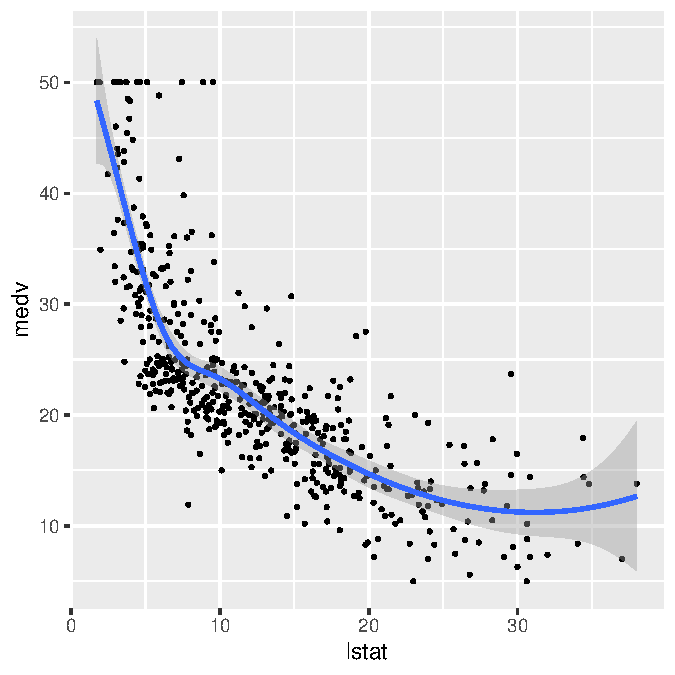
\includegraphics[width=\maxwidth]{figure/unnamed-chunk-10-1} 

\end{knitrout}


\end{document}
